% coding:utf-8

%----------------------------------------
%FOSAMATH, a LaTeX-Code for a mathematical summary for basic analysis
%Copyright (C) 2013, Daniel Winz, Ervin Mazlagic, Adrian Imboden, Philipp Langer

%This program is free software; you can redistribute it and/or
%modify it under the terms of the GNU General Public License
%as published by the Free Software Foundation; either version 2
%of the License, or (at your option) any later version.

%This program is distributed in the hope that it will be useful,
%but WITHOUT ANY WARRANTY; without even the implied warranty of
%MERCHANTABILITY or FITNESS FOR A PARTICULAR PURPOSE.  See the
%GNU General Public License for more details.
%----------------------------------------

% coding:utf-8
\section{Definition Differentialgleichungen}
Gleichungen, in der eine Variable, eine von dieser Variable abhängige Funktion 
und Ableitungen beliebigen Grades dieser Funktion vorkommen, werden 
Differentialgleichungen genannt. 
\[ F(x, y, y', y'', \ldots, y^{(n)})=0 \]
$x$ heisst dabei unabhängige und $y$ abhängige Variable. Dafür können auch 
andere Buchstaben als $x$ und $y$ verwendet werden. 
Ableitungen nach t werden auch als $\dot{y}$ geschrieben. 

\section{Grundbegriffe}

\subsection{Ordnung}
Die Ordnung einer Differentialgleichung wird durch die höchste vorkommende 
Ordnung der Ableitungen von $y$ bestimmt. 

\subsection{Grad}
Der Grad einer Differentialgleichung wird durch die höchste vorkommende Potenz 
von $y$ oder den Ableitungen von $y$ bestimmt. Potenzen der unabhängigen 
Variable werden dabei nicht berücksichtigt. 
\subsubsection*{Achtung:}
$y \cdot y' \quad \rightarrow \quad$ Grad 2

\subsubsection{Grad 1}
Differentialgleichungen vom Grad 1 nennt man linear. 

\subsection{Lösungen}
Eine Gleichung der Form
\[ F(x, y, y', y'', \ldots, y^{(n)})=0 \]
besitzt eine allgemeine Lösung. Diese enthält $n$ Parameter ($n$-parametrige 
Kurvenschar). Jede Kombination dieser Parameter ergibt eine spezielle bzw. 
partikuläre Lösung. Durch das Festlegen spezieller Werte für 
$y, y', y'', \ldots, y^{(n)}$ an einer beliebigen Stelle $x_0$ erhält man Werte 
für die $n$ Parameter und somit eine partikuläre Lösung. 

\section{Richtungsfeld und Trajektorien}
Ein Richtungsfeld ist ein Abbild einer Differentialgleichung im Raum.
Dabei wird jedem Punkt im Raum eine Steigung (\emph{Differential})
zugewiesen. Im folgenden ein Beispiel eines solchen Richtungsfeldes.

\begin{figure}[h!]
	\centering
	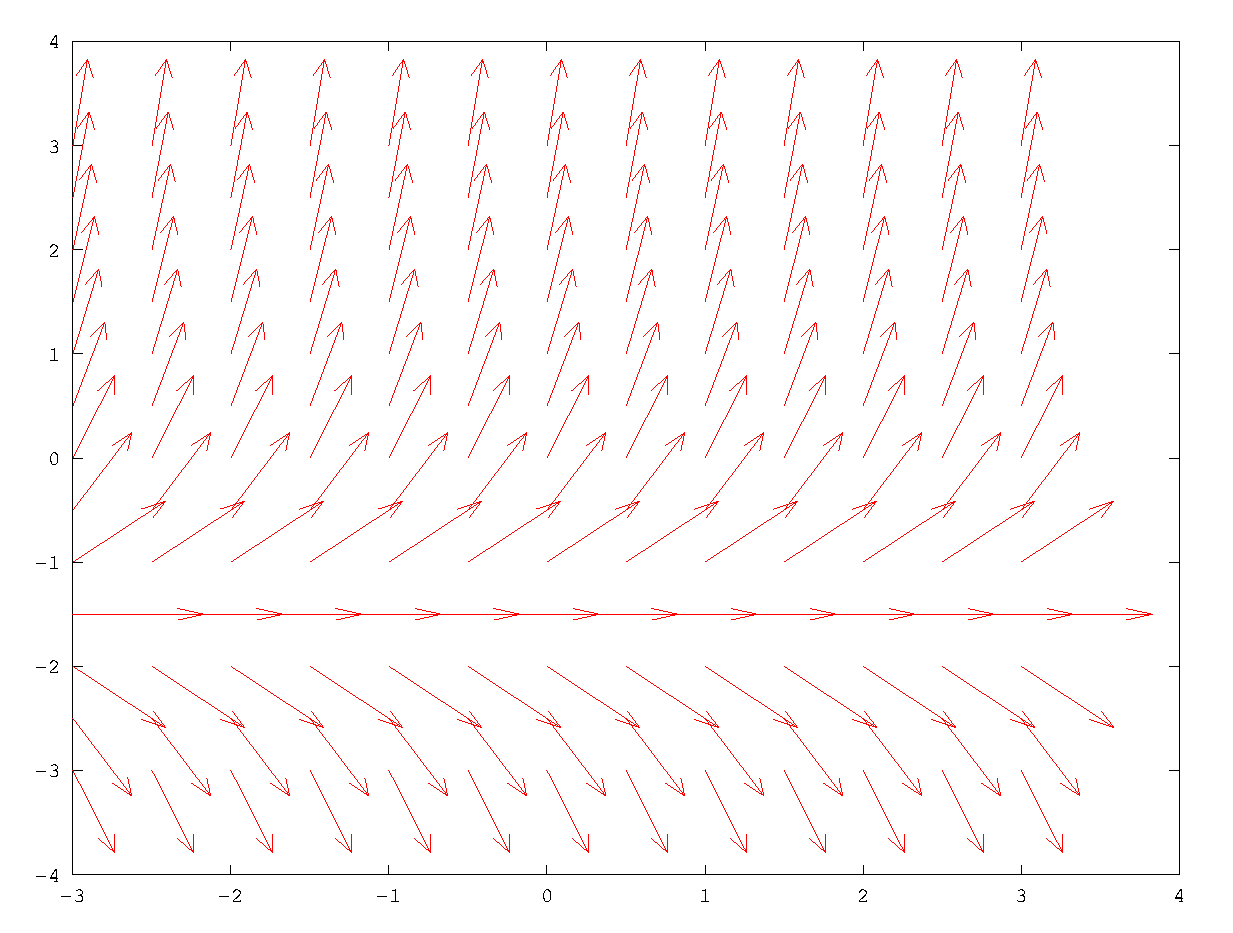
\includegraphics[width=0.8\textwidth]{field.eps}
	\caption{Richtungsfeld der Differentialgleichung $y'=3+2y$}
\end{figure}

\noindent
Die Berechnung der einzelnen Punkte erfolgt durch reines einsetzen.
Z.B. für den Punkt $P(x=1, y=-1)$ ergibt sich $3+2(-1)=1$ usw.

\subsection{Trajektorien}
Trajektorien sind Bahnkurven die die Lösung einer Differentialgleichung
darstellen. Es handelt sich dabei um eine Kurvenschar, welche eine andere
Kurvenschar mit immer dem selben Winkel schneidet. Wenn dieser Winkel
$90^{\circ}$ beträgt, so nennt man diese othogonale trajektorie.
Um eine solche orthogonale Trajektorie zu berechnen kann in drei Schritten
vorgegangen werden.
\begin{enumerate}
  \item Differentialgleichung der Kurvenschar aufstellen in der Form
	$y'=g(x,y)$
  \item Differentialgleichung der orthogonalen Trajektorien bilden
	mit Hilfe der Regel, dass $m_2=-\frac{1}{m_1}$ für orthogonale
	Kurven ist. Somit ergibt sich $y'=-\frac{1}{g(x,y)}$
  \item Allgemeine Lösung der im zweiten Schritt erstellten
	Differentialgleichung finden (z.B. mit \emph{Trennung der Variablen}
	oder \emph{Variation der Konstanten}). Diese Lösung ist dann die 
	eigentliche Trajektorie.
\end{enumerate}

\begin{figure}[h!]
	\centering
	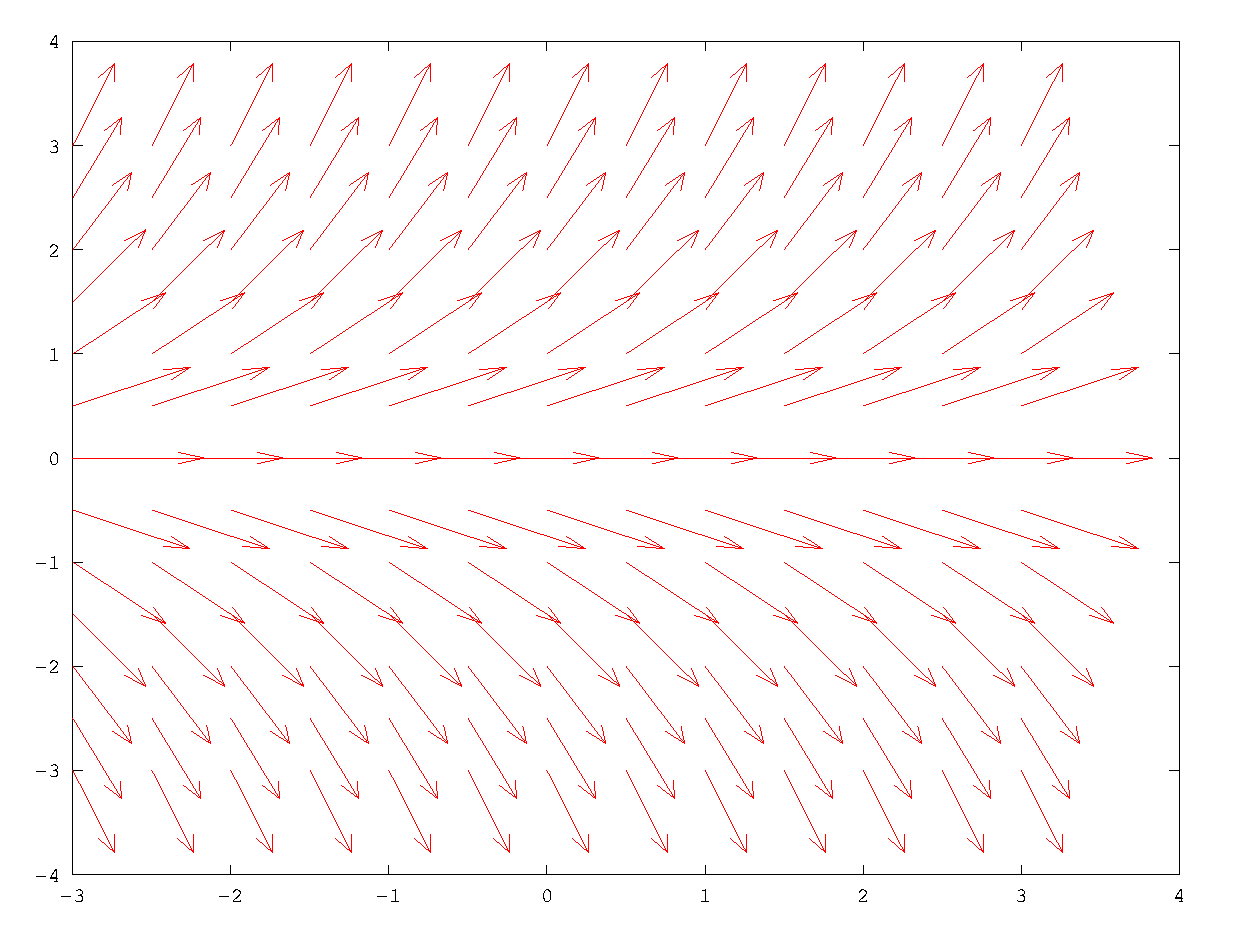
\includegraphics[width=0.48\textwidth]{trajektorien1.eps}
	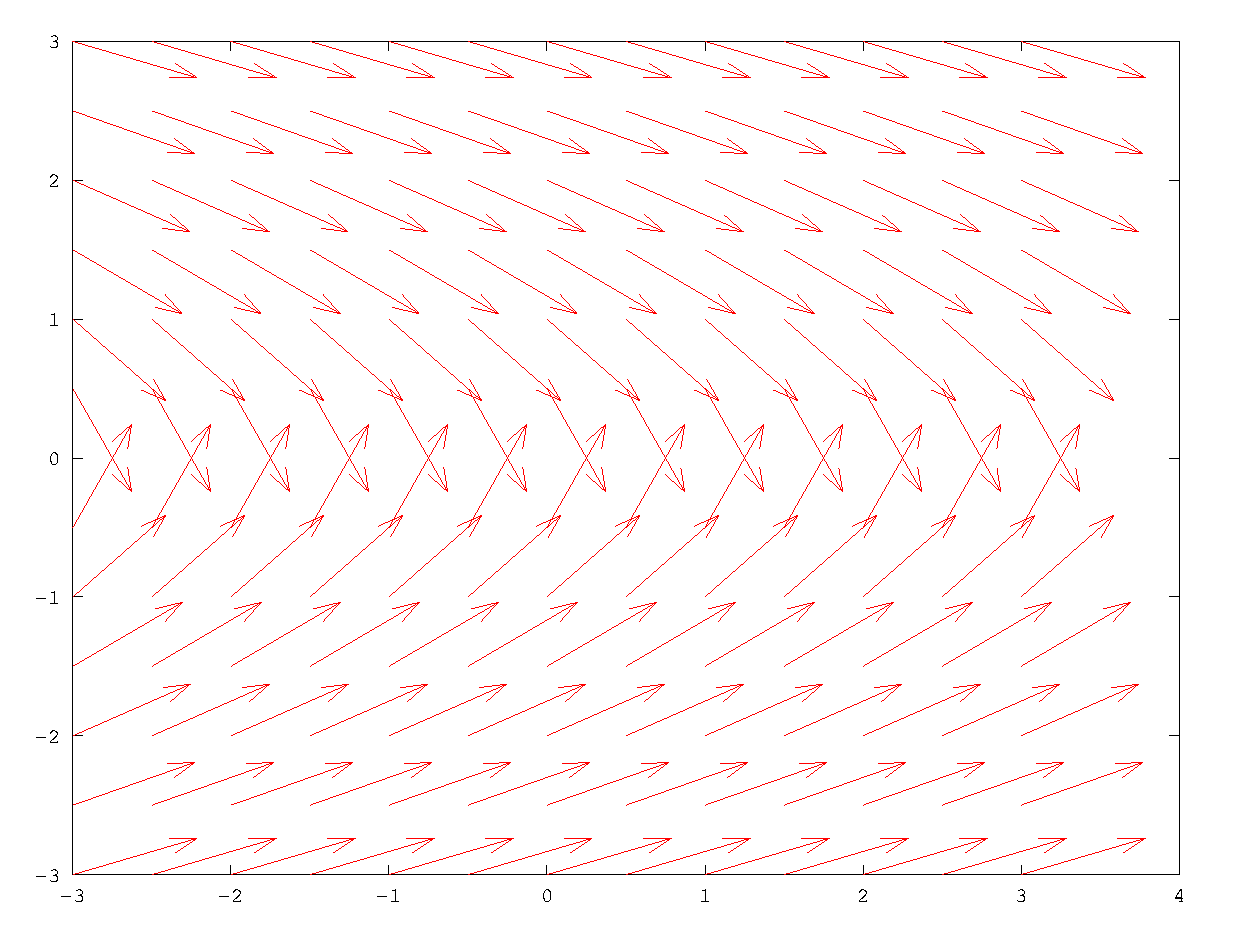
\includegraphics[width=0.48\textwidth]{trajektorien2.eps}
	\caption{Normale Kurvenschar (links, $y'=y$) 
	und orthogonale Trajektorie (rechts, $y'=-\frac{1}{y}$)}
\end{figure}

\section{Lösungsverfahren}

\subsection{Variation der Konstanten \\(Lineare Gleichung 1. Ordnung)}
\begin{enumerate}
  \item Inhomogene Gleichung notieren / aufstellen (I)
  \item Normalform bilden / aufstellen (N)
  \item Homogene Gleichung bilden / aufstellen (H)
  \item $g(x)$ und $G(x)$ bestimmen ($G(x) = \int g(x)$)
  \item $G(x)$ einsetzen in die allgemeine Lösung $y_h=c \cdot e^{-G(x)}$
        $\rightarrow$ so erhält man die allgemeine Lösung der 
        homogenen Gleichung (H)
  \item Variation der Konstanten d.h. aus dem c wird eine Funktion $K(x)$ 
        $(\rightarrow y= \ldots)$
  \item Funktion ableiten (für $y'$)
  \item Die neuen Definitionen für $y$ und $y'$ einsetzen in die Normalform (N) 
  \item Auflösen nach $K(x)$ (durch Integration)
  \item Einsetzen in die allgemeine Lösung der homogenen Gleichung ($y_h$)
\end{enumerate}

\newpage

\section{Lineare Differentialgleichungen zweiter Ordnung}
Spricht man von linearen Differentialgleichungen zweiter Ordnung, 
so heisst dies, dass die abhängige Variable zweifach abgeleitet
vorkommt.
\[ a\cdot y'' + b \cdot y' + c \cdot y = \tilde{s}(x) 
   \qquad \text{allgemeine Form}\]
\[ y'' + a_1 \cdot y' + a_0 \cdot y = s(x) 
   \qquad \text{Normalform}\]
   \[  s(x) \neq 0 \qquad \text{Inhomogen} \]
   \[  s(x) \neq 0 \qquad \text{Homogen} \]

\subsection{Homogene Gleichung}
Zwei Funktionen $y_1(x)$ und $y_2(x)$ heissen linear unabhängig falls
\[ y_1(x)=c \cdot y_2(x) \qquad \text{oder} \qquad y_2(x)=c \cdot y_1(x) \]
wobei $c$ eine Konstante ist. Anderenfalls heissen $y_1(x)$ und $y_2(x)$
linear unabhängig.

\subsubsection{Satz}
\begin{itemize}
  \item Sind $y_1(x)$ und $y_2(x)$ Lösungen der homogenen Gleichung,
	so ist die neue Funktion 
	\[ y(x) = c_1y_1(x) + c_2y_2(x) \]
	wieder eine Lösung der homogenen Gleichung, wobei $c_1, c_2$
	beliebige Konstanten sind.
  \item Sind $y_1(x)$ und $y_2(x)$ linear unabhängige Lösungen der 
	homogenen Gleichung, so ist
	\[ y=c_1y_1 + c_2y_2 \qquad c_1, c_2 \in \mathbb{R} \]
	die allgemeine Lösung der homogenen Gleichung.
\end{itemize}

\subsubsection{Lösungsverfahren}
Um eine lineare homogene Differentialgleichung zweiter Ordnung zu 
lösen, kann wie folgt vorgegenagen werden.
\begin{enumerate}
  \item Homogene Gleichung sinngemäss notieren
	\[ y'' + a_1y' + a_0y = 0 \]
  \item Charakteristische Gleichung aufstellen.\\
	Der Ansatz hierzu: $y=e^{kx}$ somit ist $y'=k\cdot e^{kx}$
	und $y''=k^2 \cdot e^{kx}$.
	\[ k^2 + a_1k + a_0 = 0 \]
  \item Gleichung nach $k$ auflösen mit der Formel
	\[ k_{1,2} = \frac{1}{2}\left( -a_1 \pm \sqrt{a_1^2 - 4a_0} \right)  \]
  \item Diskriminante betrachten und entsprechend einsetzten
	\begin{itemize}
	  \item $D > 0$ zeigt zwei reelle Lösungen an\\
		\[ y=c_1e^{k_1x} + c_2e^{k_2x} \]
          \item $D = 0$ zeigt zwei gleiche reelle Lösungen an\\
		\[ y=c_1e^{kx} + c_2xe^{kx} \]
          \item $D < 0$ zeigt zwei komplexe Lösungen an\\
		\[ y=c_1e^{\mu x} cos(\omega x) + c_2e^{\mu x} sin(\omega x) \]
		\[ k=\mu + j \omega \]
		Wie es zu einer komplexen Lösung kommt: 
		Wenn die Diskriminate $D < 0$ ist, so kann der Wurzelausdruck
		statt z.B. $\sqrt{-25}$ als 
		$\sqrt{(-1)25}=\sqrt{-1}\sqrt{25}=j5$ geschrieben werden.
		Dies wäre dann das $j\omega$ aus obiger Formel.
	\end{itemize}
\end{enumerate}

